\documentclass[twoside]{AiTeX}



\title{PEV}
\author{A.L.K.}
\date{Diciembre 2021}
\begin{document}
%\datos{facultad}{universidad}{grado}{asignatura}{subtitulo}{autor}{curso}
\datos{Informática}{Universidad Complutense de Madrid}{Ingeniería informática}{Programación Evolutiva}{Memoria de la práctica 2}{Alejandro Barrachina Argudo \\ Adrià Carreras Bagur }{2023}
\portadaApuntes
\pagestyle{empty}
\tableofcontents
\pagestyle{empty}
\justify
\pagestyle{fancy}

\newpage

\chapterA{Capturas de funcionamiento}

\begin{figure}[H]
    \centering
    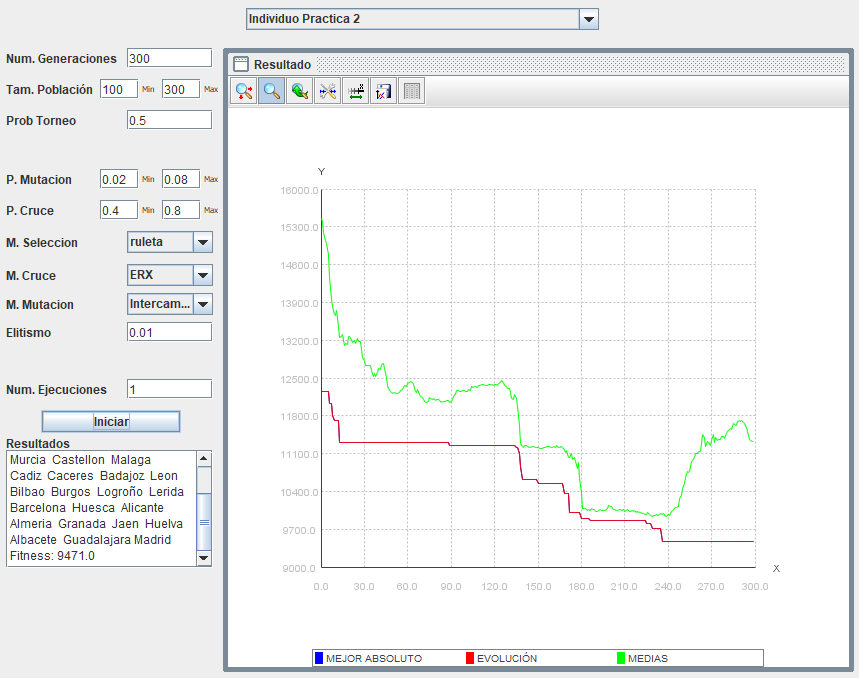
\includegraphics[width = \textwidth]{Images/Captura1.png}
    \caption{Captura 1}
    \label{fig:1}
\end{figure}

Se puede ver el funcionamento de la práctica con los valores predeterminados, con un resultado por debajo de los 10.000.

\begin{figure}[H]
    \centering
    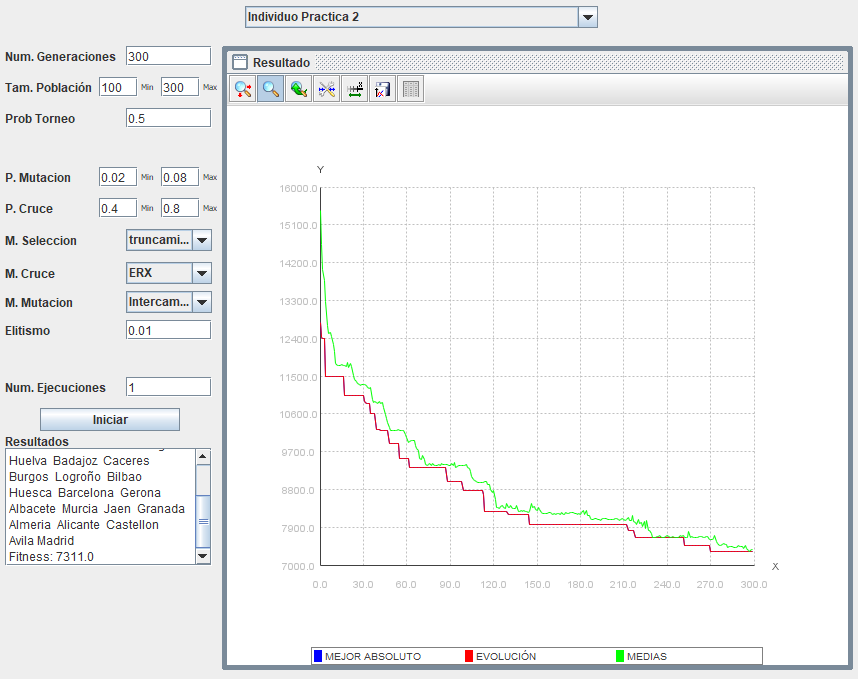
\includegraphics[width = \textwidth]{Images/Captura2.png}
    \caption{Captura 2}
    \label{fig:2}
\end{figure}

Solamente cambiando el método de selección a truncamiento se pueden notar mejoras, con una muy buena evolución.

\begin{figure}[H]
    \centering
    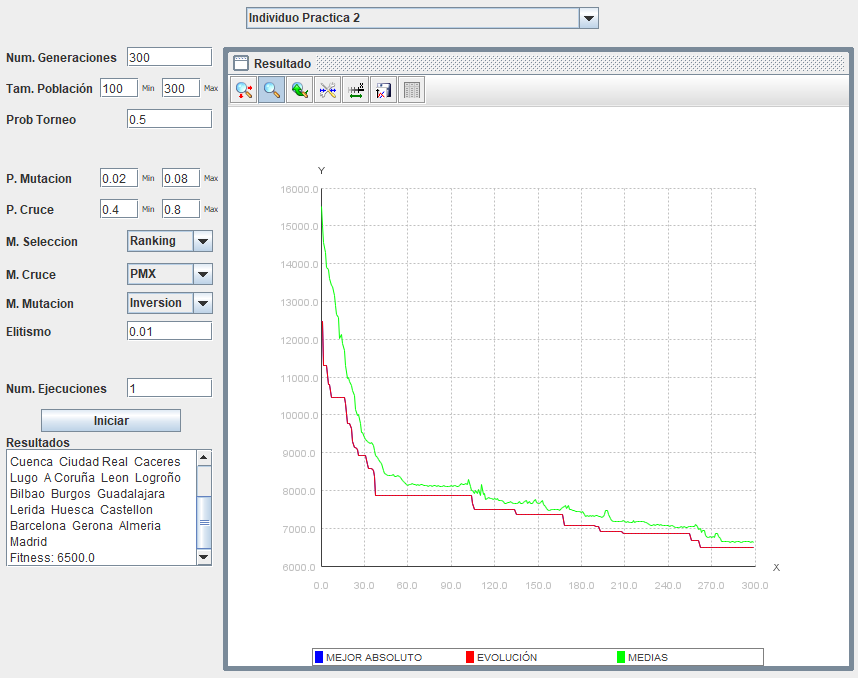
\includegraphics[width = \textwidth]{Images/Captura3.png}
    \caption{Captura 3}
    \label{fig:3}
\end{figure}

El método de Ranking consigue muy buenos resultados, juntándolo con el cruce PMX y la mutación por inversión es extremadamente eficiente y preciso.

\begin{figure}[H]
    \centering
    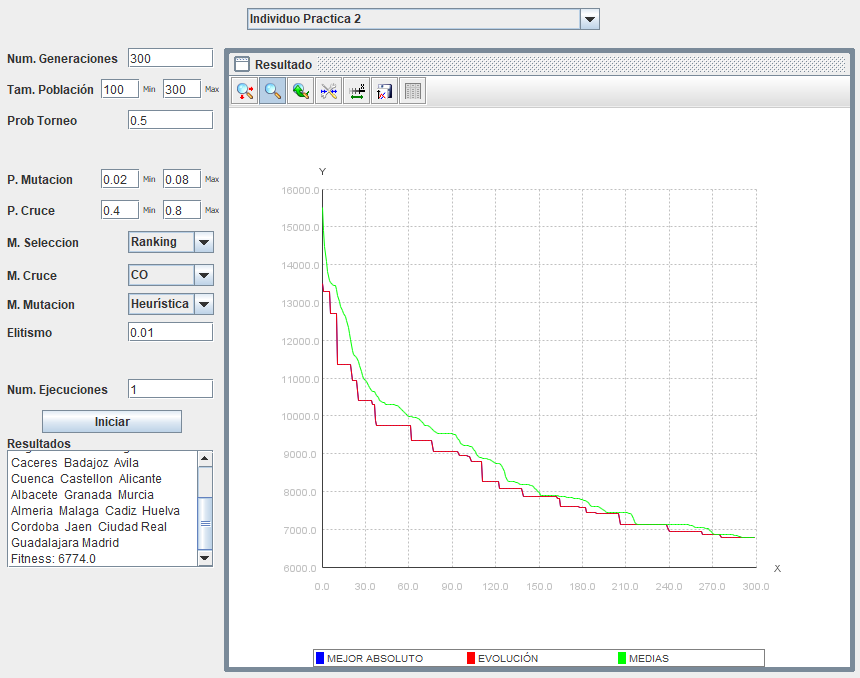
\includegraphics[width = \textwidth]{Images/Captura4.png}
    \caption{Captura 4}
    \label{fig:4}
\end{figure}

La mutación heurística da también muy buenos resultados aunque sacrificando eficiencia.

\begin{figure}[H]
    \centering
    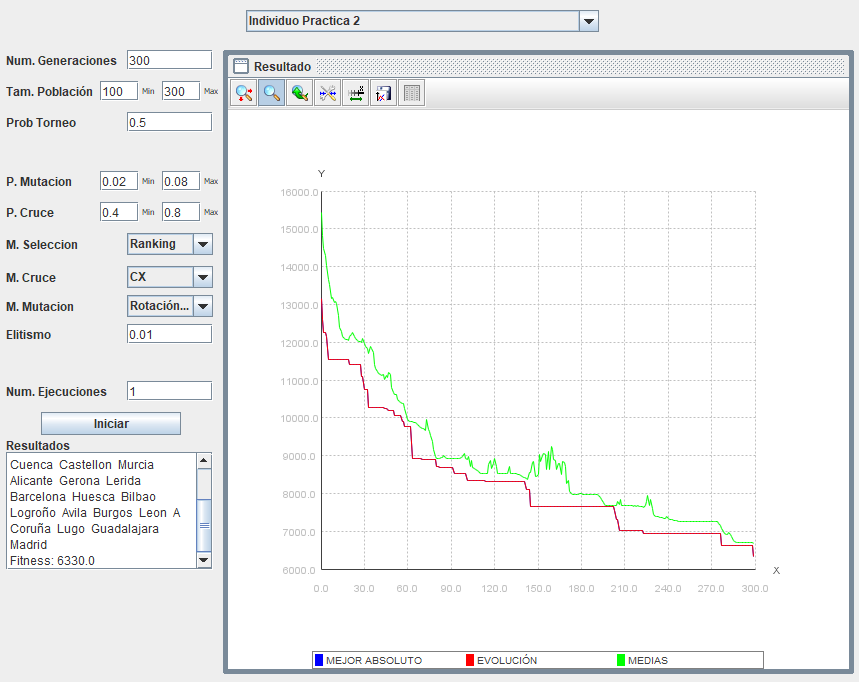
\includegraphics[width = \textwidth]{Images/Captura5.png}
    \caption{Captura 5}
    \label{fig:5}
\end{figure}

Nuestro método propio rotación heurística consigue resultados similares al anterior, también sacrificando eficiencia.

\begin{figure}[H]
    \centering
    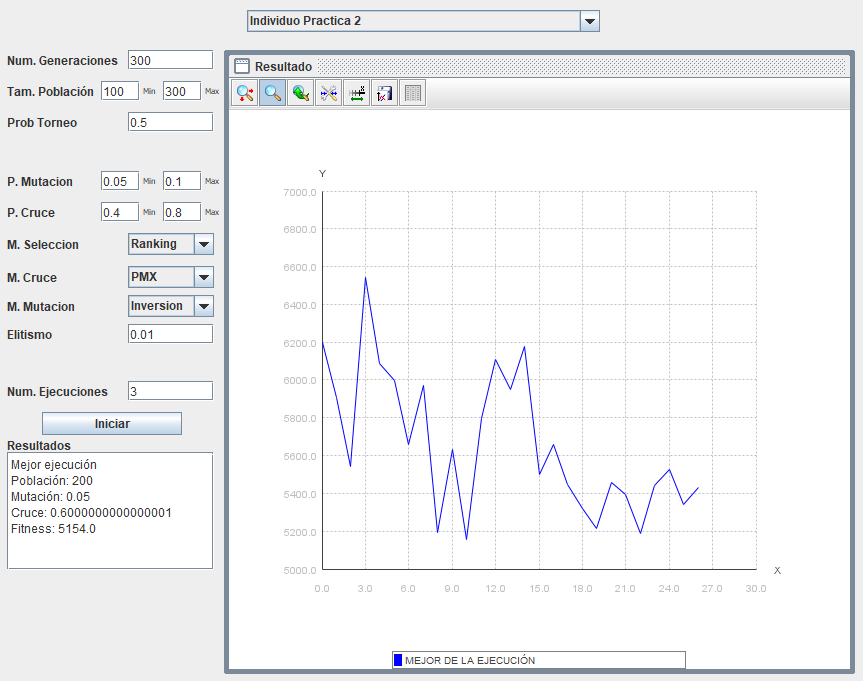
\includegraphics[width = \textwidth]{Images/Captura6.png}
    \caption{Captura 6}
    \label{fig:6}
\end{figure}

Con varias ejecuciones se consiguen resultados excepcionales.

\begin{figure}[H]
    \centering
    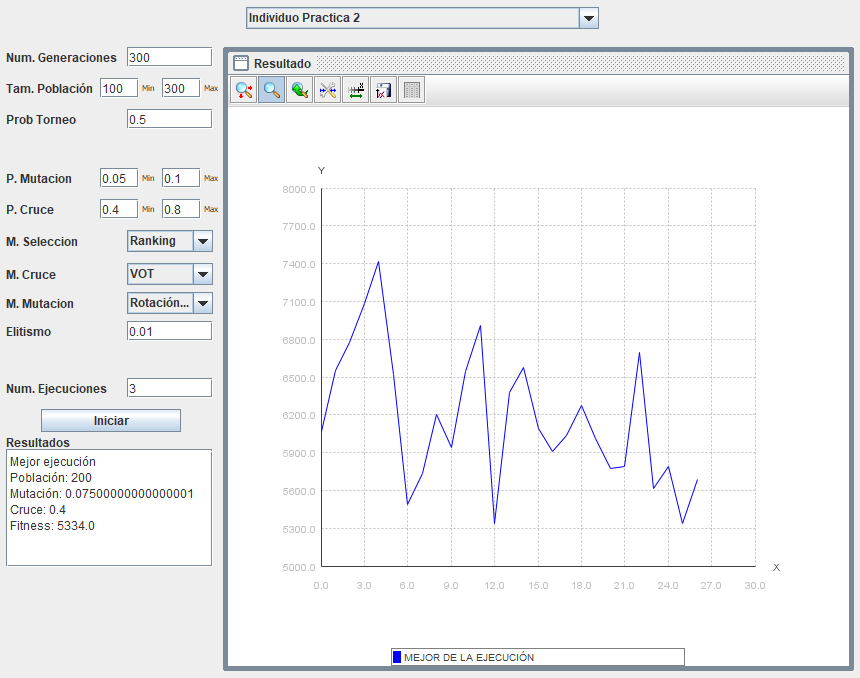
\includegraphics[width = \textwidth]{Images/Captura7.png}
    \caption{Captura 7}
    \label{fig:7}
\end{figure}

Se puede observar que no es común que el mejor resultado se dé con la máxima población, se consigue juntando unos bunos parámetros de cruce y mutación.

\chapterA{Observaciones de la práctica, arquitectura del código y ejecución}

\section{Observaciones}

Los métodos de selección que mejores resultados nos han dado han sido: truncamiento y ranking. El truncamiento, el más eficiente puede tener el peligro de quedarse estancado en algún punto, aunque con un buen uso de los cruces y la mútacion es excepcional, véase la figura \ref{fig:2}.
El método de ranking se desarrolla de manera muy parecida a la de truncamiento siendo más estable, véase la figura \ref{fig:3}.

Los métodos de cruce más efectivos han sido PMX, CX, CO y VOT. Destacan entre sus compañeros por lo capaces que son de dar el mejor resultado en el mínimo número de generaciones, entre ellos la diferencia no es tan notoria. Véanse las figuras \ref{fig:3}, \ref{fig:5}, \ref{fig:4}.
Nuestro método propio VOT arroja muy buenos resultados, aunque sacrificando eficiencia por el uso de randoms, véase la figura \ref{fig:7}.

Las mejores mutaciones que se han usado han sido la de inversión, heurística y el método propio rotación heurística. Siendo inversión la que destaca por su eficiencia.

\section{Arquitectura}

Para mantener todo el código organizado, se usa la siguiente estructura de paquetes:

\begin{itemize}
    \item\textbf{go2:} paquete que engloba toda la práctica.
    \item\textbf{g02.cruces:} Paquete que reúne los cuatro cruces distintos bajo la interfaz Cruces.
    \item\textbf{g02.individual:} Paquete que contiene todos los individuos de las distintas funciones bajo la clase padre Individuo<T>.
    \item\textbf{g02.Selections}: Paquete para reunir las distintas selecciones usadas en la práctica bajo la clase padre Selection<T>, donde se encuentra las funciones para corregir el fitness.
    \item\textbf{g02.Ventana}: Paquete para la interfaz gráfica de la práctica y el método main.
\end{itemize}

Para una visión mas completa del proyecto, desde el navegador puede abrir el archivo G02/target/site/index.html

\section{Métodos Propios}

Cruce VOT: Inspirado en el cruce por votación, dados dos padres se seleccionan los genes que sean iguales y que ocupen la misma posición en ambos, estos genes pasan directamente a los dos hijos en la misma posición que ocupaban.
A continuación, siguiendo desde el último gen insertado, los hijos se reparten aleatoriamente los genes de los padres en cada posición. Hijo1[x] e Hijo2[x] se reparten los genes Padre1[x] y Padre2[x] de manera aleatoria.
Si tras el paso anterior no se ha completado alguno de los hijos, se inserta el resto al igual que en el cruce por orden.

Mutación de Rotación Heurística: Inspirada en la mutación por rotación y heurística, dada una subcadena aleatoria en el cromosoma, ésta se va a mantener de la misma forma, los genes fuera de la subcadena van rotando a la derecha y calculando el fitness hasta que se vuelva a la misma posición, se devuelve el cromosoma que haya obtenido el mejor fitness.

\section{Ejecución y compilación de la práctica}

Al ser un proyecto en maven se puede importar directamente desde eclipse con la opción de abrir proyectos del sistema de archivos.

Para compilar el proyecto solo hay que darle al botón de \textit{run} y debería instalar las dependencias necesarias. Si no fuera así se puede ejecutar el comando \textit{mvn install} para instalar todas las dependencias.

Así mismo, el proyecto se puede correr desde el propio eclipse usando el botón de \textit{run}, usando la configuración de \textit{aplicación java} y como clase principal g02.Ventana.ventana.

El archivo jar se encuentra en la carpeta P01/target/


\chapterA{Distribución de trabajo y conclusiones}

\section{Distribución}

Adrià ha hecho la GUI, los cruces OXPP, CX, ERX, CO, las mutaciones por inversión, inserción y heurística y los métodos propios. Alejandro ha hecho la implementación y la codificación del individuo, el método de selección ranking, los cruces OX, PMX y OXOP y la mutación por intercambio.

\section{Conclusiones}

En conclusión, para enfrentarse a este problema es necesario dedicar más generaciones, dada la alta cantidad de soluciones posibles, lo que hace que debamos tener en cuenta la eficiencia más que nunca.

Los métodos de selección que mejores resultados nos han dado han sido: Truncamiento y Ranking, siendo el Truncamiento el más efectivo, aunque más propenso a quedarse estancado.

Las mutaciones han sido muy útiles y pueden afectar mucho al resultado, siendo las mejores: Inversión, Heurística y Rotación Heurística, la primera la más eficiente al no tener que calcular el fitness.




\end{document}
